



\begin{frame}
  \begin{block}{Antena}
    \begin{center}
      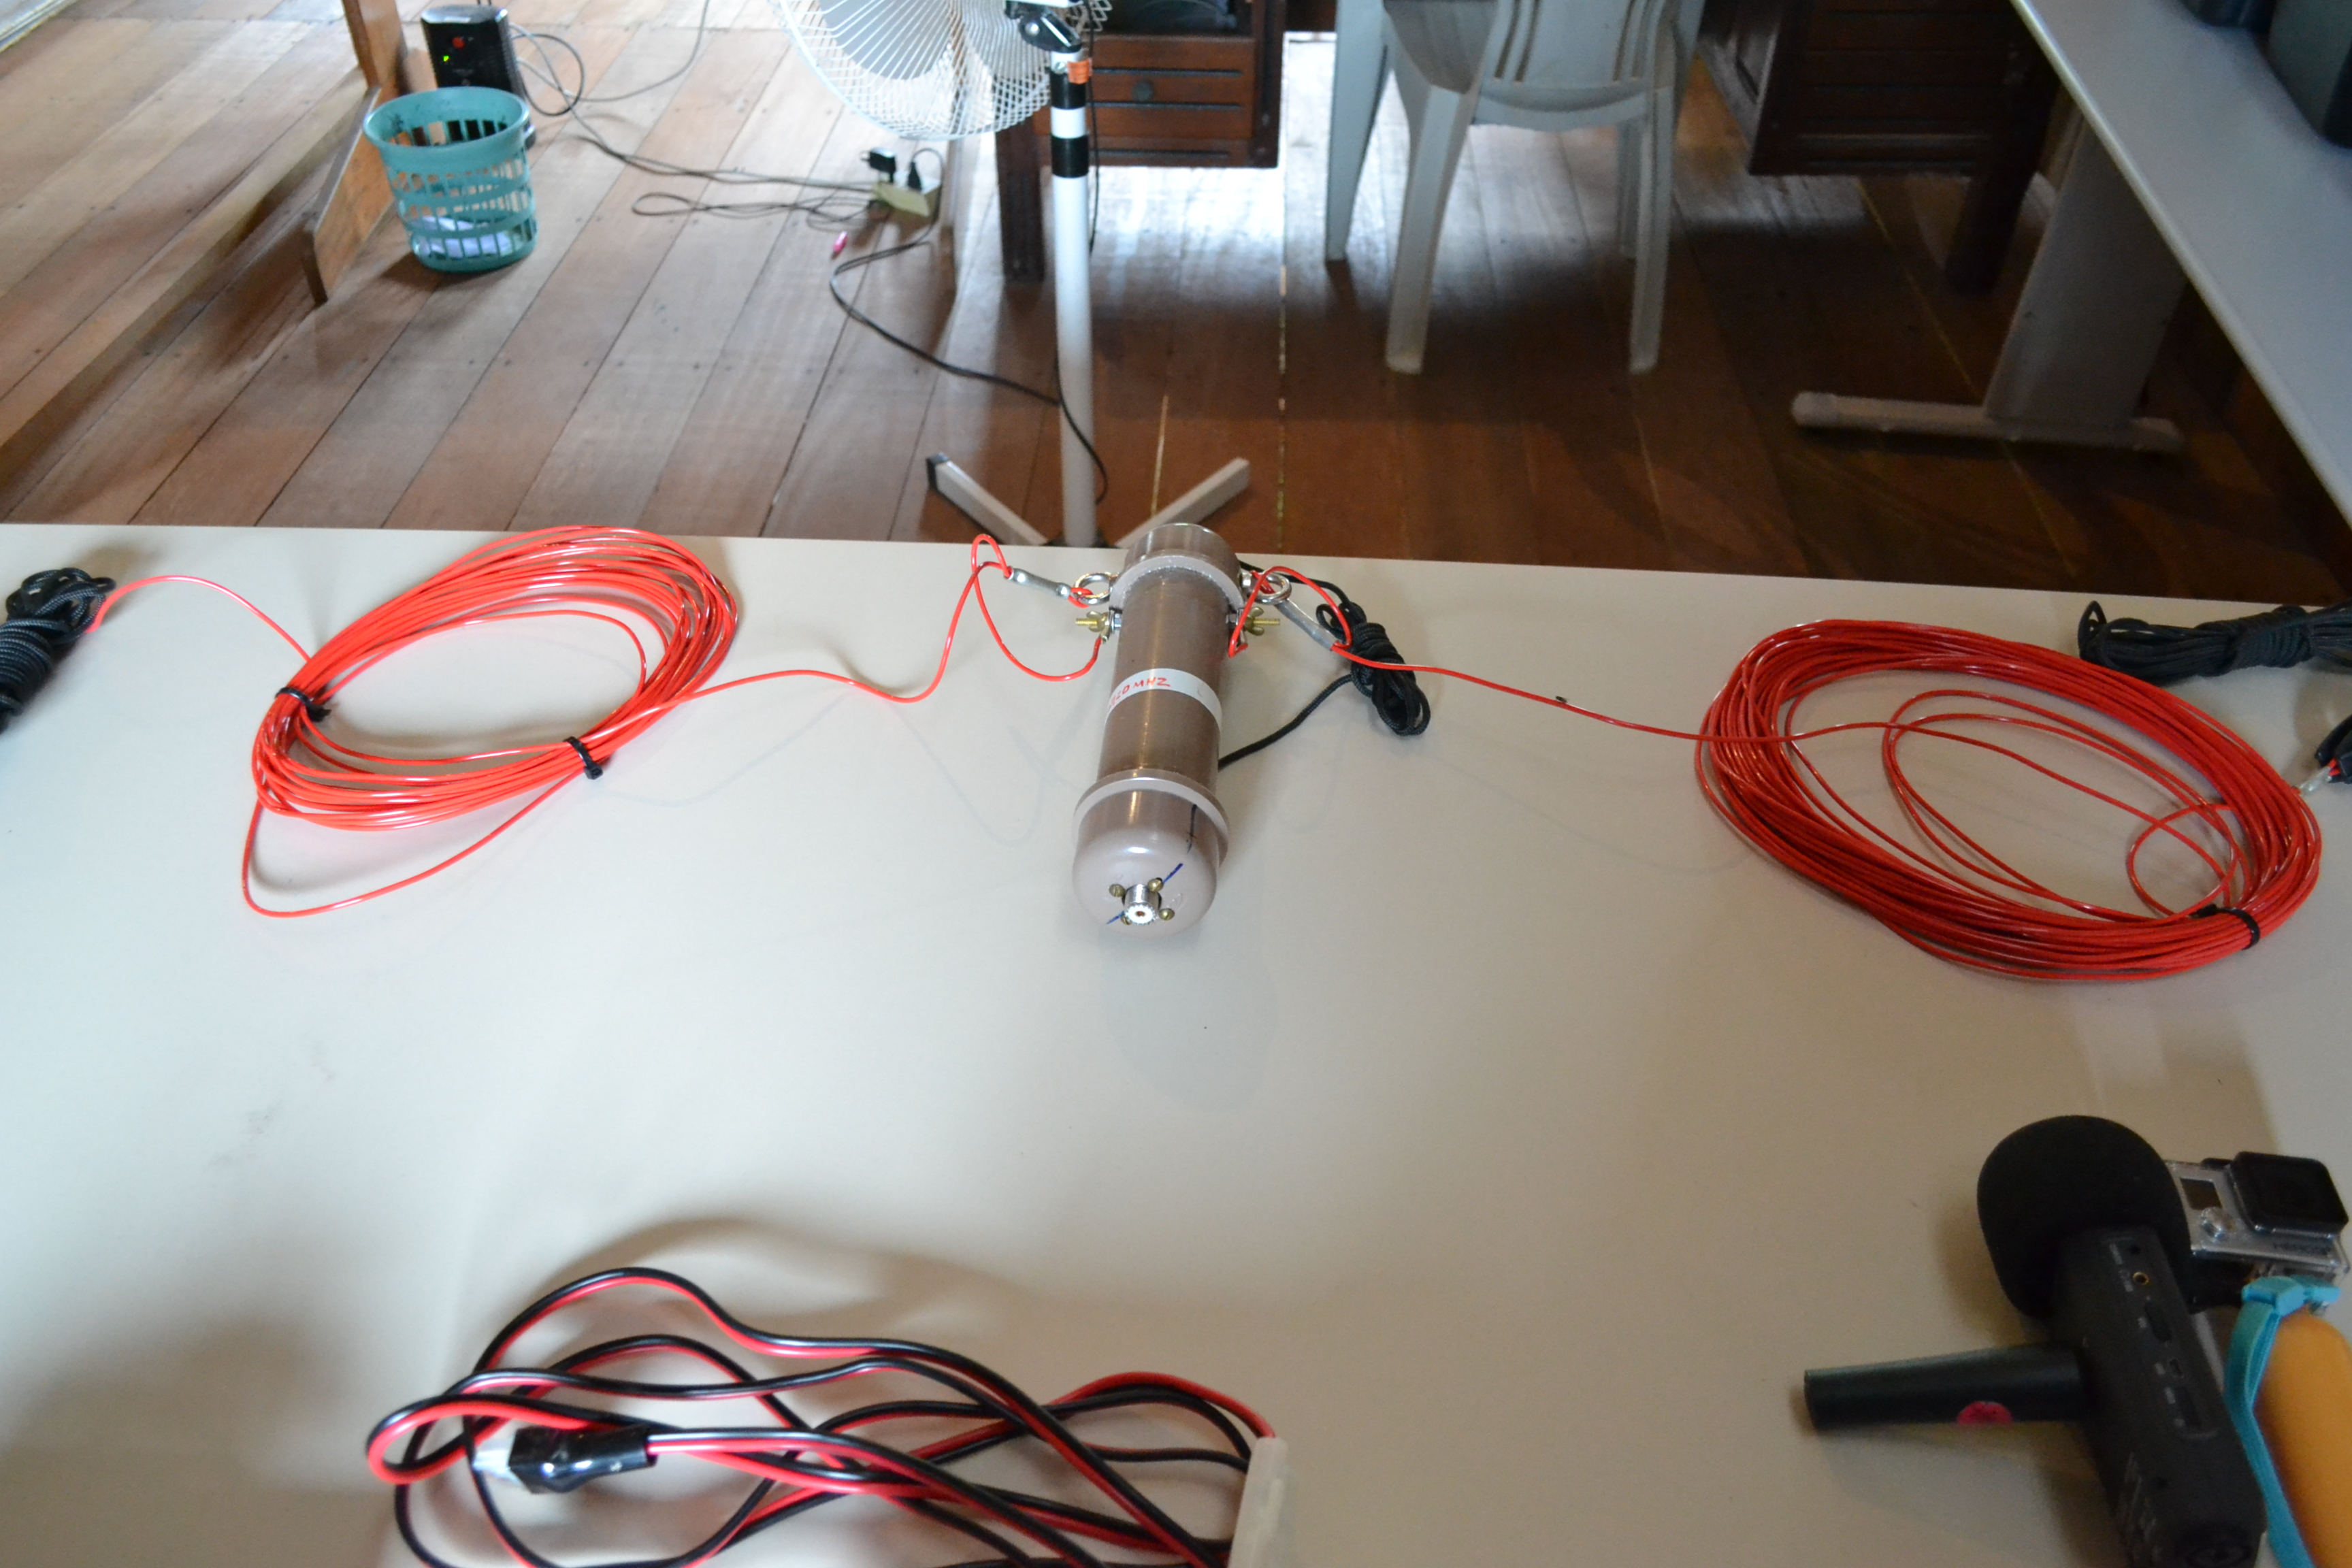
\includegraphics[width=.7\columnwidth]{antena.jpg}
    \end{center}
  \end{block}

\end{frame}

\begin{frame}
  \begin{block}{Painel solar}
    \begin{center}
      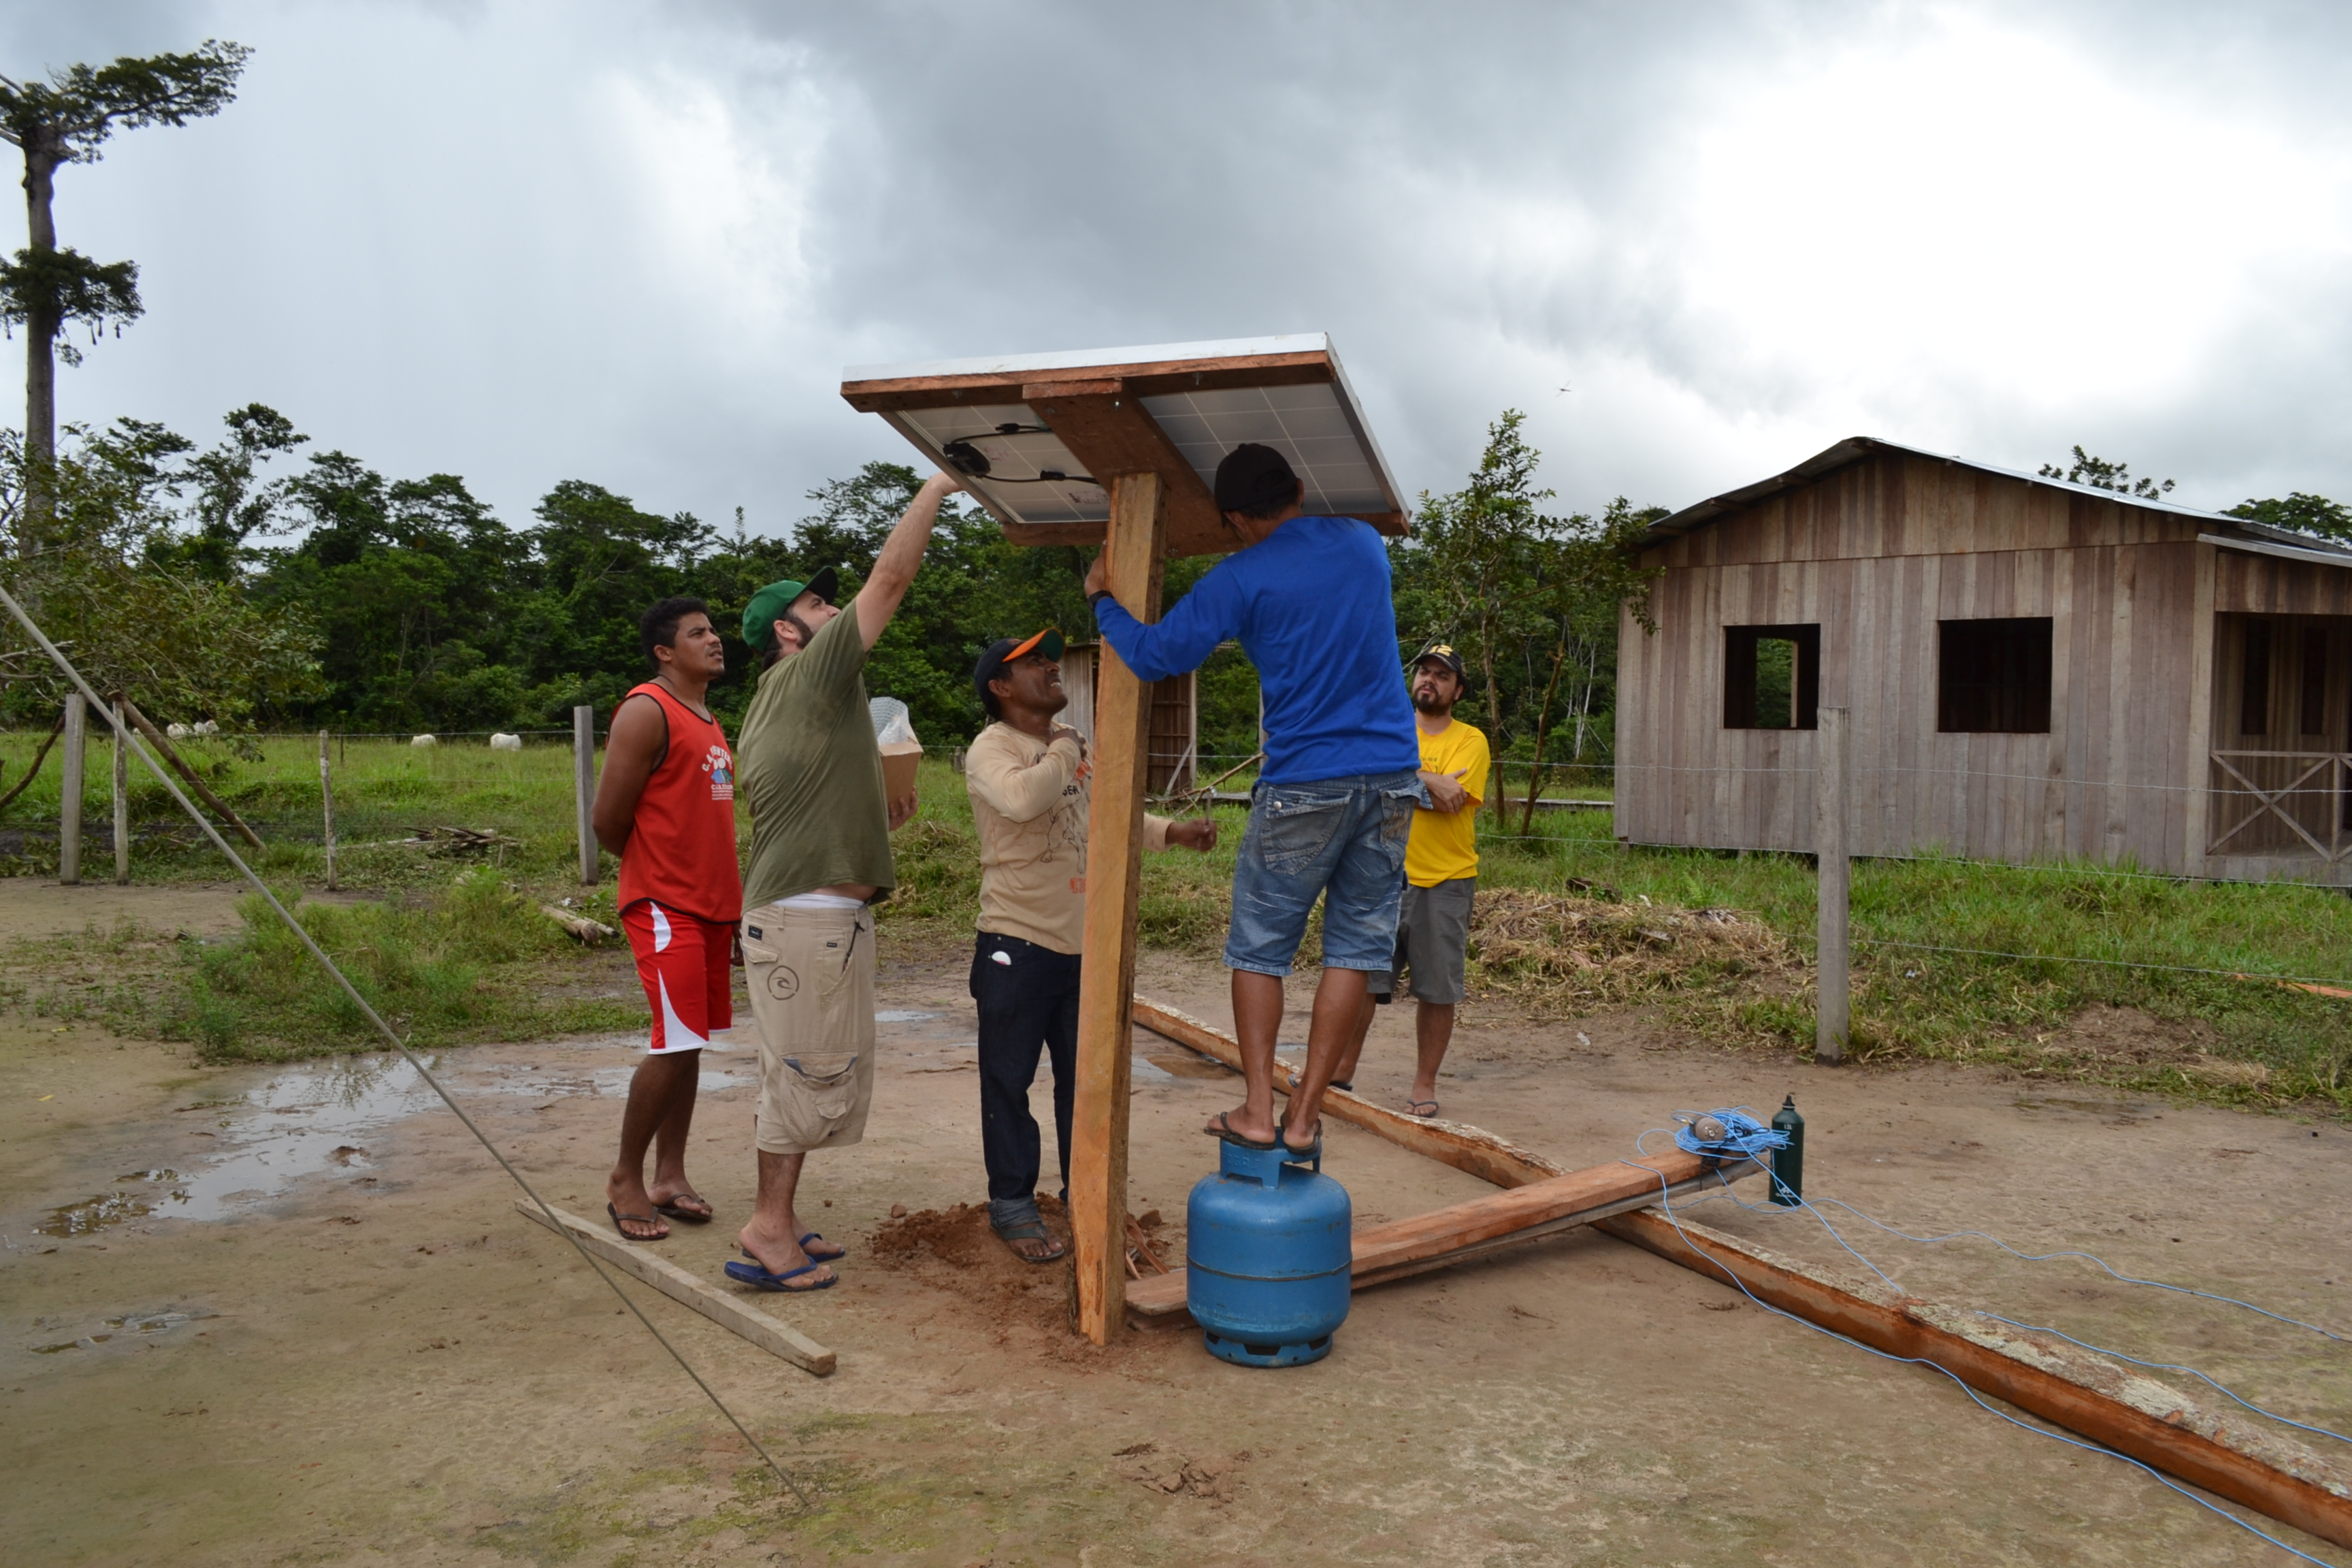
\includegraphics[width=.7\columnwidth]{solar.jpg}
    \end{center}
  \end{block}

\end{frame}

\begin{frame}
  \begin{block}{Transceptor HF}
    \begin{center}
      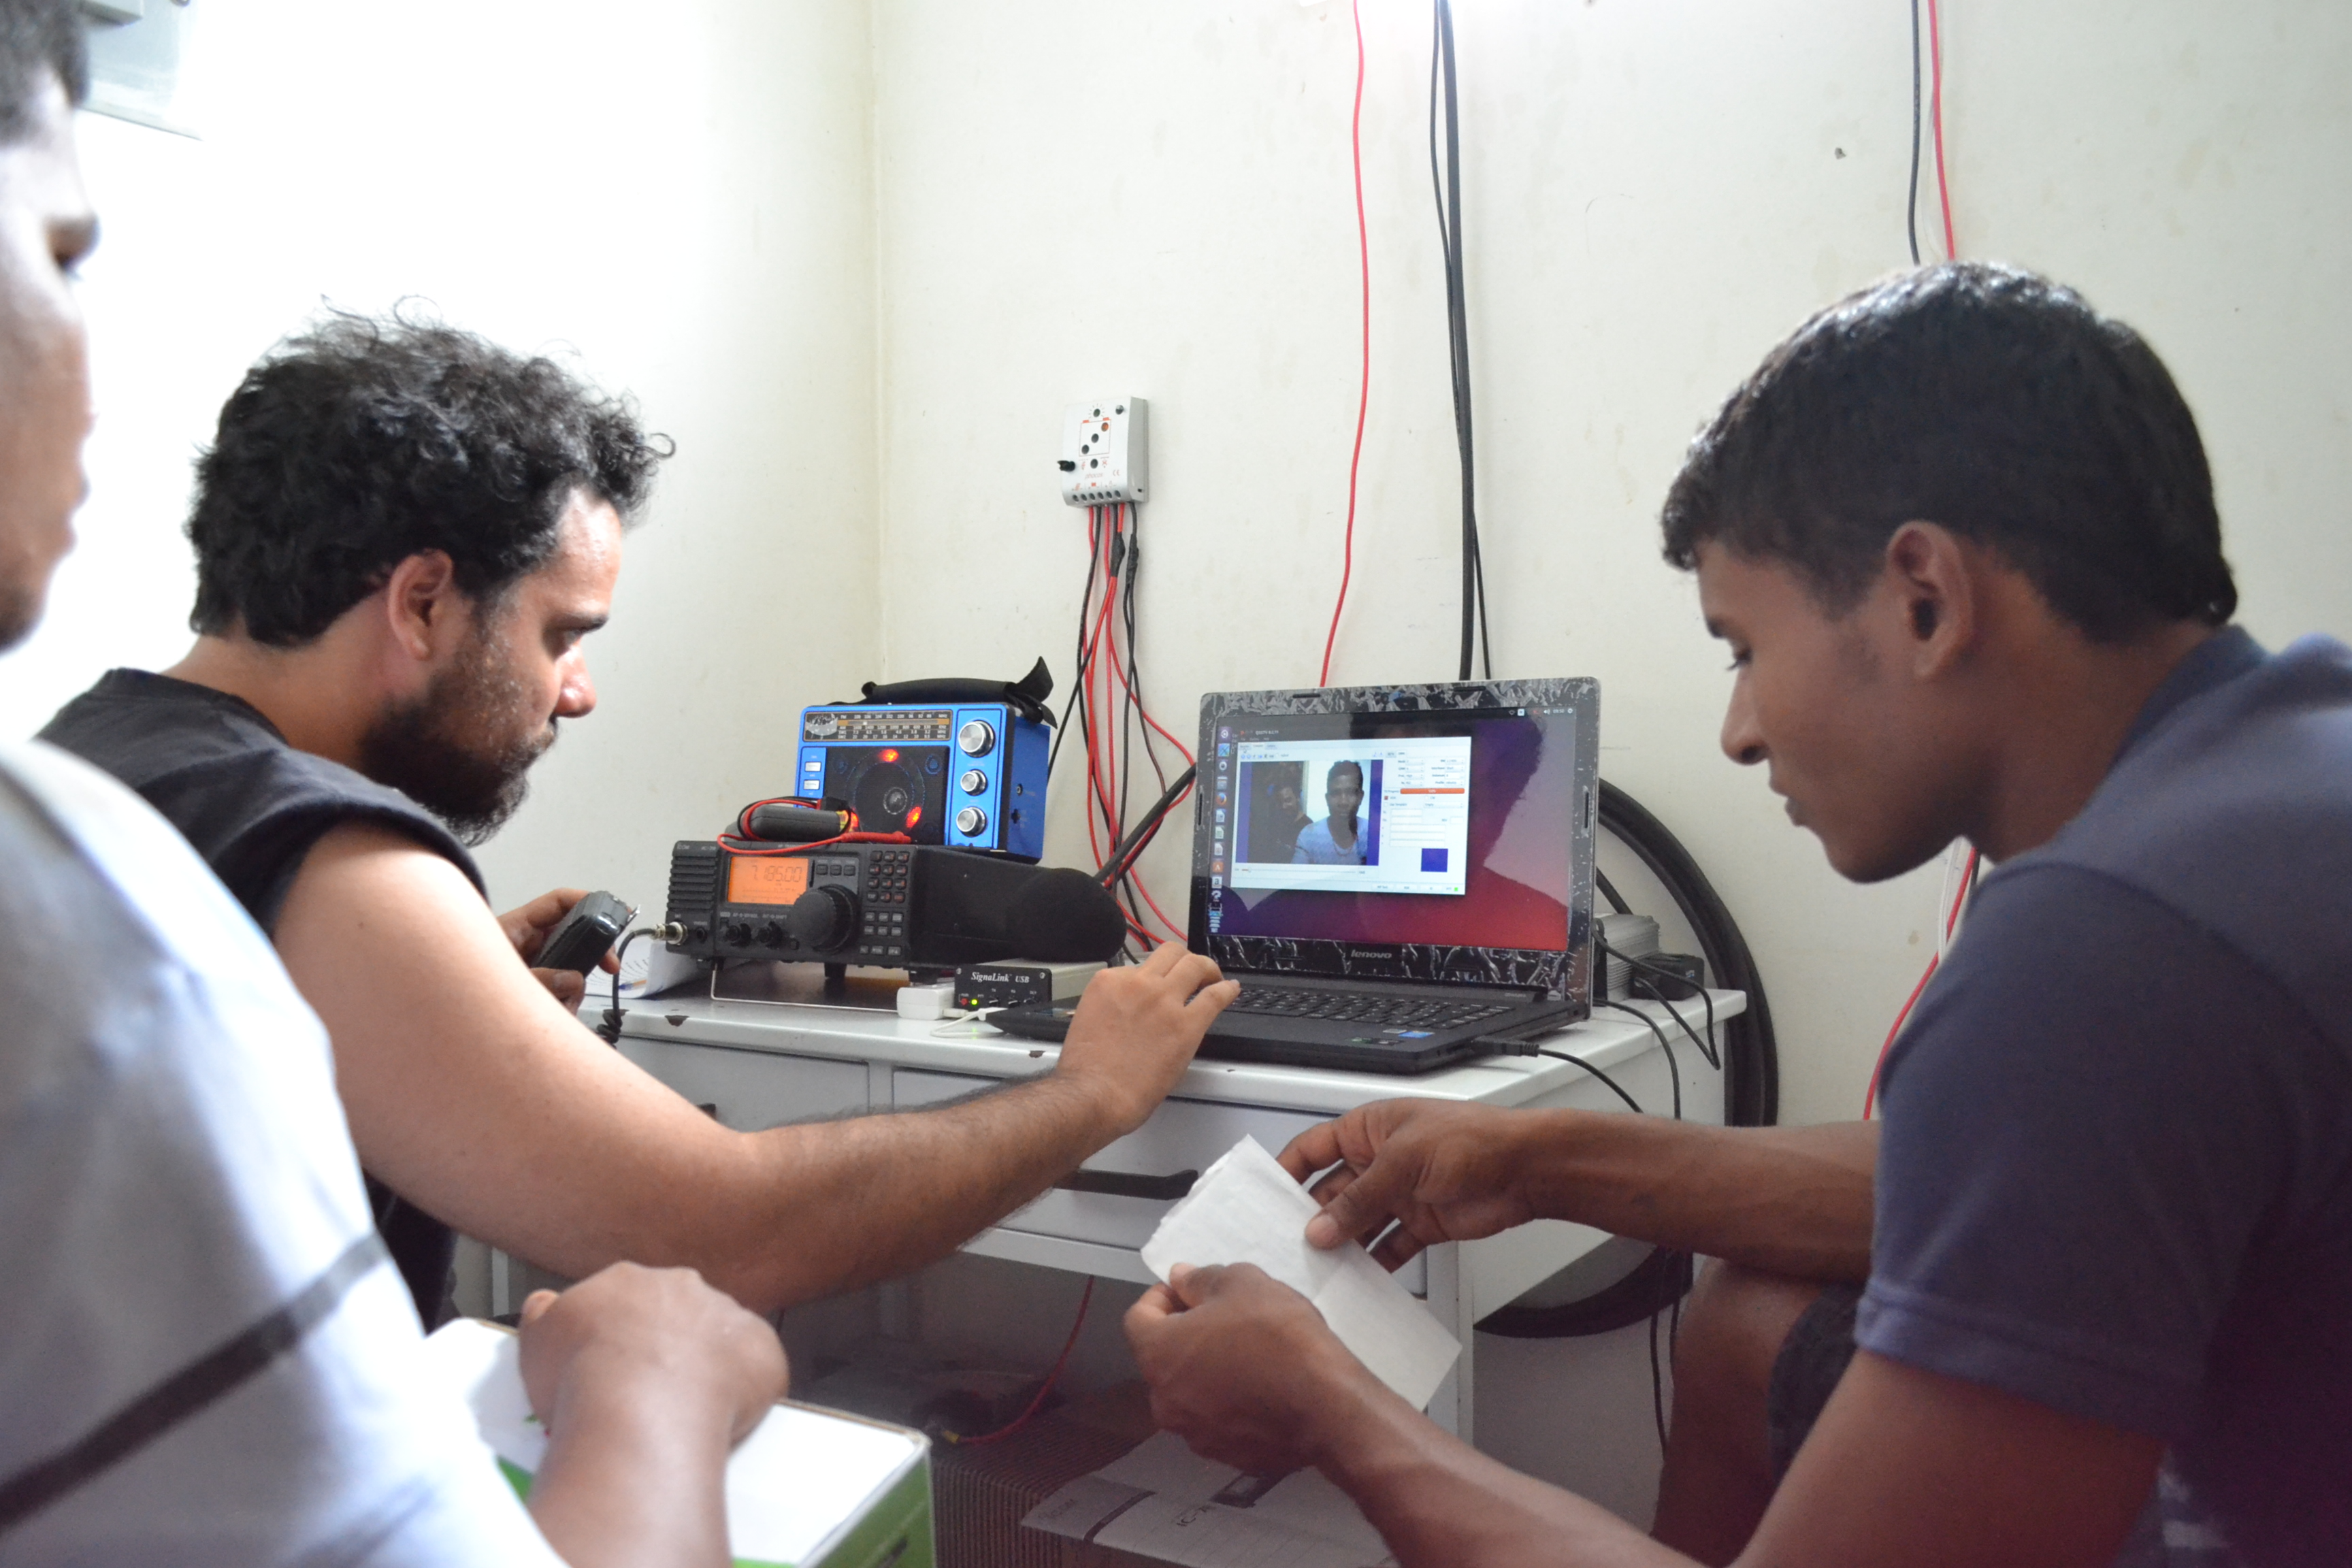
\includegraphics[width=.7\columnwidth]{config.jpg}
    \end{center}
  \end{block}
\end{frame}


\begin{frame}
  \begin{block}{Pilha de rede para uso civil do HF}
    \begin{itemize}
      \item Modems HF disponíveis precisam ter banda menor que 3 kHz
      \item Uso do protocolo IP - sérios desafios
      \item Protolocos mais adaptados para uso em HF: UUCP (Proj. HERMES)
    \end{itemize}
  \end{block}

  \begin{center}
    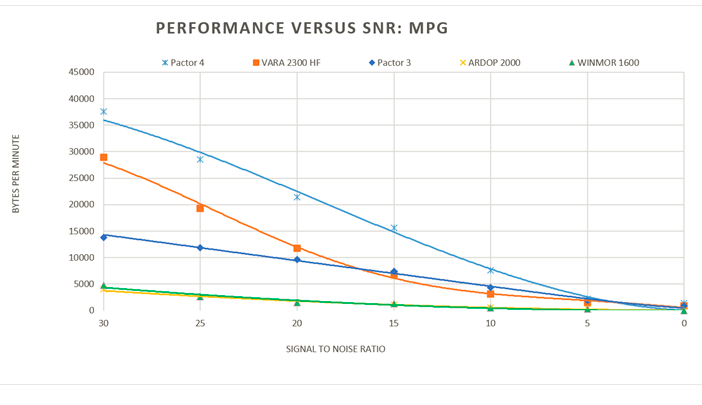
\includegraphics[width=.65\columnwidth]{image_modems.png}
  \end{center}

\end{frame}

\begin{frame}
  \begin{block}{Novos codificadores de sons e imagens}
    \begin{itemize}
      \item Codificadores de voz baseados em aprendizado de máquina de 450 a 3000 bps, eg. LPCNet e Lyra;
      \item Codificadores de imagem de última geração
        (eg. H.266, EVC), ou baseados em aprendizado de máquina, eg. HiFiC
    \end{itemize}
  \end{block}

\end{frame}



\begin{frame}

\begin{block}{Telecom em HF - Conclusões}

  \begin{itemize}
  \item Grande assimetria tecnológica entre sistemas de telecomunicações HF
    militares e civis
  \item Sistemas militares - larguras de banda maiores (até 48~kHz)
  \item Sistemas civis - limitação de 3kHz
  \item Carência de transceptores de banda larga para uso civil
  \item Uma pilha de rede otimizada para uso civil em HF pode impulsionar a
    adoção da banda HF para telecomunicação digital
\end{itemize}
\end{block}

\end{frame}


\begin{frame}
\begin{block}{Radiodifusão em HF}


  \begin{itemize}
  \item Testes de rádio digital em HF no Brasil (MCTI, EBC, UnB, BT)
  \item Transmissão digital em HF - DRM em 11.910 kHz
  \item Configuração mais usada: 10 kHz BW, DRM Mode B, SDC 4 QAM, MSC 16 QAM
  \item Uso de antena HRS do parque do Rodeador, de ganho 17 dB, azimute 329°
  \end{itemize}
\end{block}

\end{frame}


\begin{frame}

  \begin{center}
    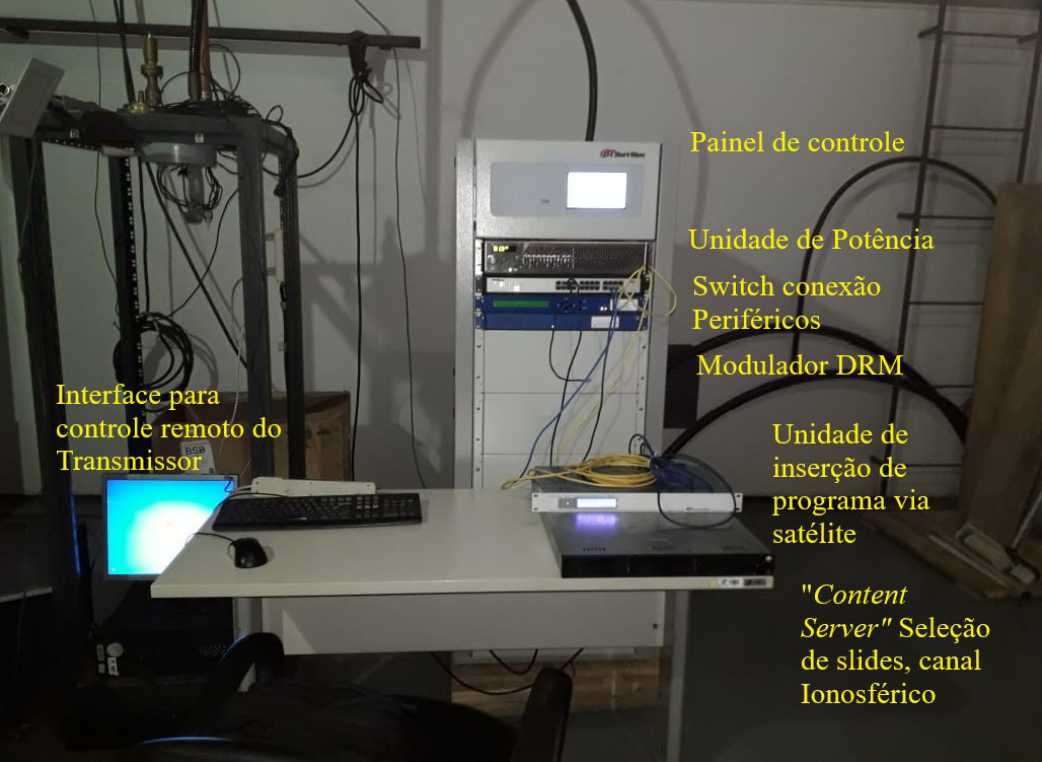
\includegraphics[width=.75\columnwidth]{im1.jpg}
  \end{center}


\end{frame}

\begin{frame}

  \begin{center}
    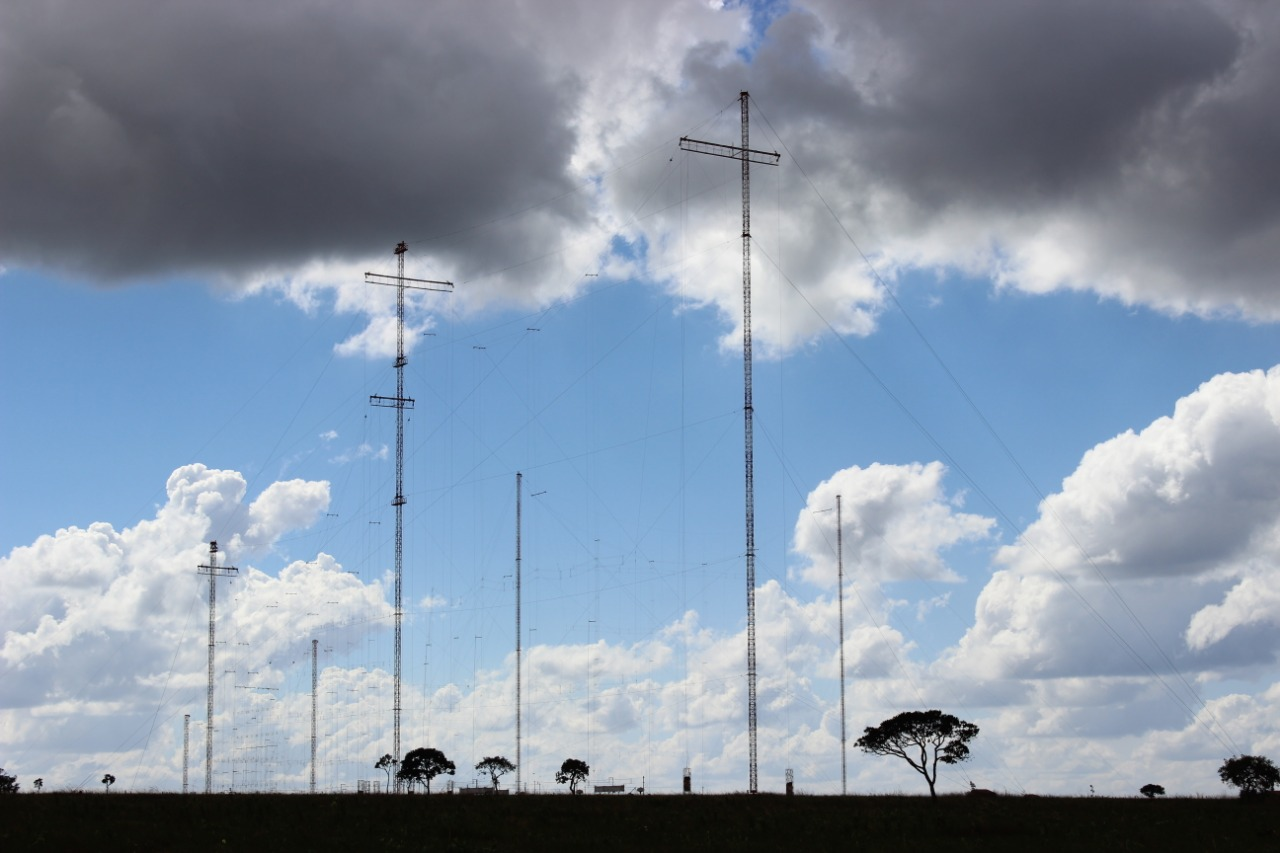
\includegraphics[width=.8\columnwidth]{rodeador.jpg}
  \end{center}

\end{frame}

\begin{frame}

    \begin{center}
      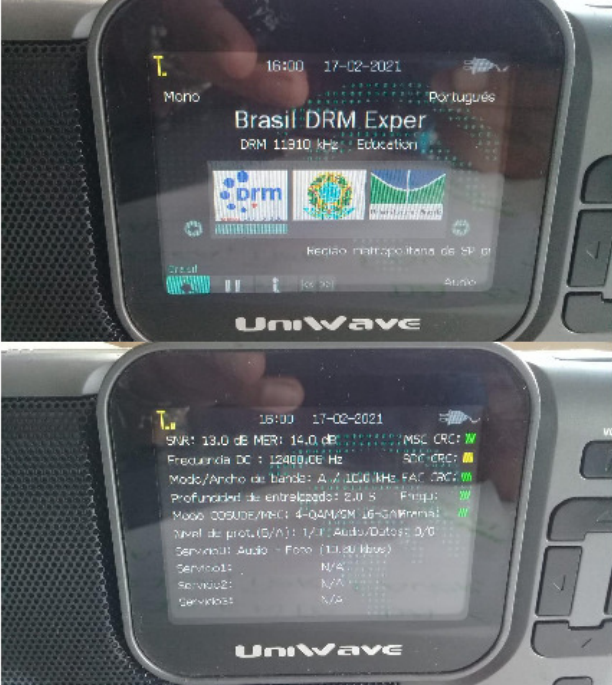
\includegraphics[width=.45\columnwidth]{radio.jpg}
    \end{center}

\end{frame}

\begin{frame}

  \begin{block}{Medidas realizadas na UFRR em Boa Vista / RR}
    \begin{center}
      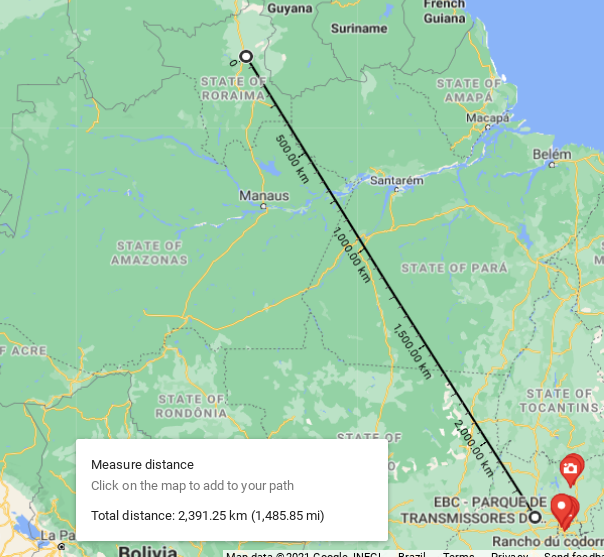
\includegraphics[width=0.5\columnwidth]{map.png}
    \end{center}
  \end{block}

\end{frame}


\begin{frame}

  \begin{block}{Medidas realizadas na UFRR em Boa Vista / RR}
    \begin{center}
      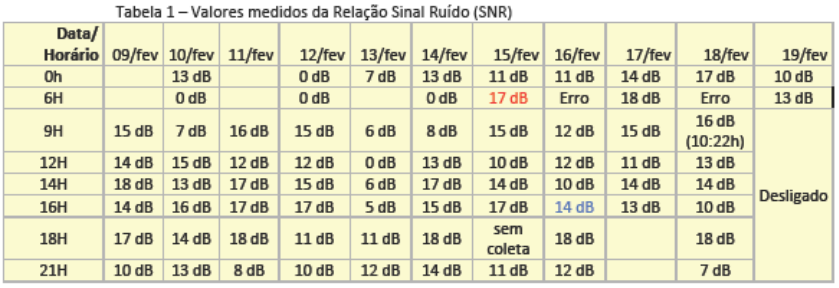
\includegraphics[width=.9\columnwidth]{snr.jpg}
    \end{center}
  \end{block}

\end{frame}


\begin{frame}

  \begin{block}{Equipe no Rodeador / EBC}

    \begin{center}
      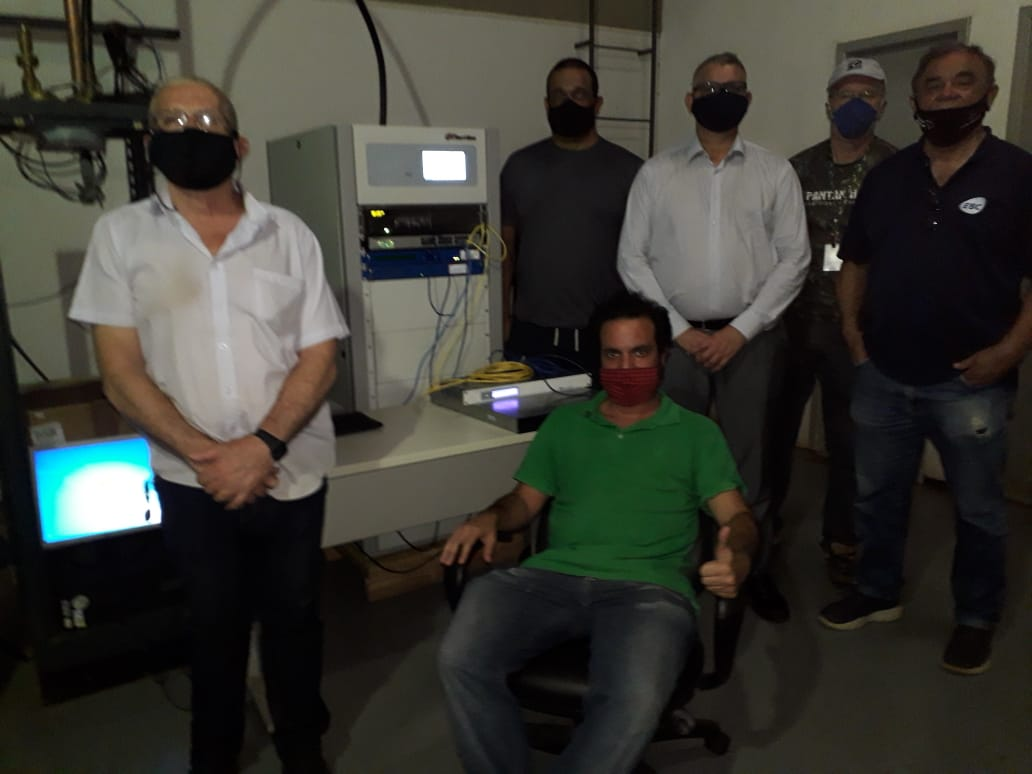
\includegraphics[width=.60\columnwidth]{foto.jpg}
    \end{center}

  \end{block}

\end{frame}


\begin{frame}

  \begin{center}
    Telecomunicação e Radiodifusão em HF apresentam soluções únicas!
  \end{center}

    \begin{center}
      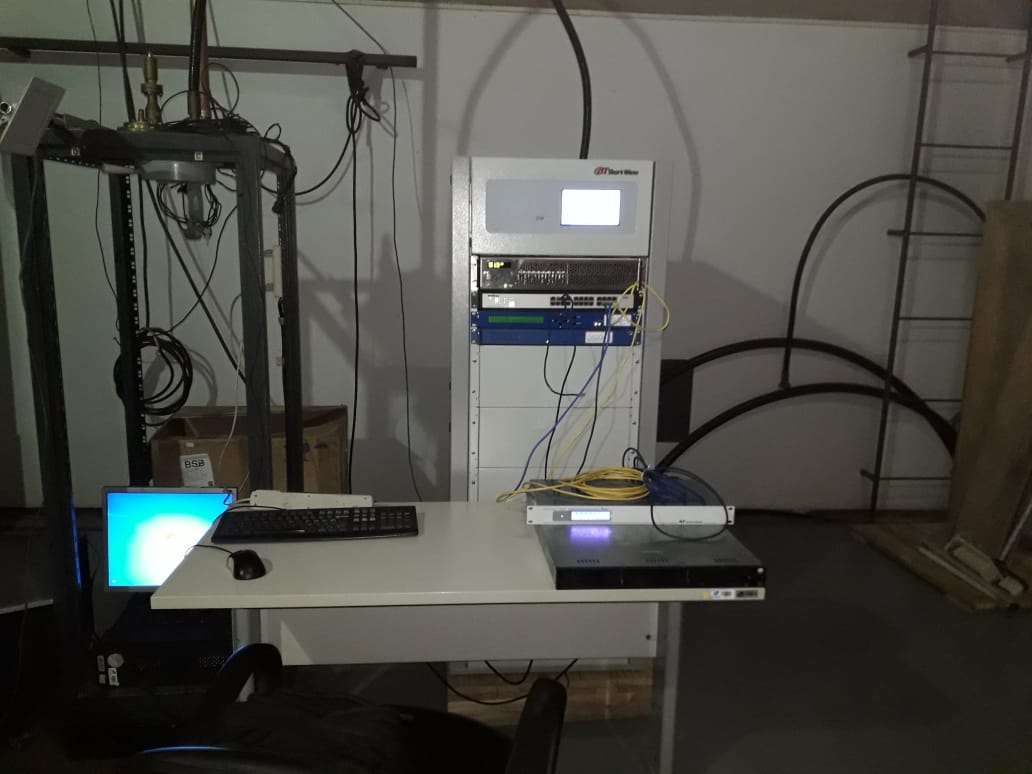
\includegraphics[width=.7\columnwidth]{foto2.jpg}
    \end{center}


\end{frame}
